\chapter{Heat Conductivity in Superfluid Helium and Heater Tests~\label{sec:heattest}~\cite{Florian_thesis}}

%The cooling process of the spallation neutrons creates a heat input on
%the cryostat. This heat input must be removed to keep the temperature
%of the superfluid helium constant. This is critical, since the storage
%lifetime of UCN depend strongly on the superfluid helium temperature.

There are several sources of heat input on the UCN cryostat such as
the cooling process or the target irradiation. The heat load on the
UCN cryostat creates a temperature gradient along the heat exchanger
to the suprefluid helium bottle~(see Fig.~\ref{fig:gasflow}. The
temperature gradient in the superfluid helium is described by its heat
conductivity. Lower heat conductivities give rise to larger
temperature gradients.

The temperature dependence of the heat conductivity in the superfluid
helium is describe by theorical models from the lambda point at 2.17~K
down to around 1.4~K which is above the temperatures for the UCN
production~($<~1$~K). Since it is difficult to reach such low
temperatures, the mechanism of heat transfer in temperatures below
1.4~K is not fully understood.  To check the validity of the
theoretical models, here the extrapolation to lower temperatures is
compared to the acquired data with the vertical UCN source.


In order to create a temperature gradient along the channel from heat
exchanger to the superfluid helium bottle, the heater tapes that are
wrapped around the superfluid helium bottle are used.
%These heaters can
%create a temperature gradient between the heat exchanger and the
%superfluid helium bottle~(see Sec.~\ref{sec:vertical_source}).
This temperature gradient can be measured using the temperature
sensors shown in Fig.~\ref{fig:TSs}.

The heater test procedure is the following; The heater tape around the
superfluid helium bottle is turned on when the temperature of the
superfluid helium is stable. Here this temperature is refered to as
the {\it{base}} temperature. The applied heat load could easily be
calculated since the applied current and voltage are known. After the
heater is turned on, the temperature of the superfluid helium starts
to increase. This causes an increase in the flow rate in the $^3$He
pot. After some time, the temperature of the superfluid helium starts
to settle and reach a new equilibrium. This temperature is referred to
as the {\it{saturation}} temperature. At this point, the heater could
be turned off which causes the superfluid temperature and the flow
rate of the $^3$He to get back to the initial conditions.

In 2017, two sets of heater tests were performed on the vertical UCN
source: The April heat test and the November heat test. In April, the
base temperature of the superfluid helium was slightly higher than in
November. In addition, there was no proton beam during the April
cooling of the cryostat and it was purely a cryostat cooling
test. Table.~\ref{tab:heattest} shows the heat load and the
temperatures of the superfluid helium for those tests.

\begin{sidewaystable}
  %\centering
  \begin{tabular}{|c|c|c|c|c|c|c|c|c|c|c|}
    \hline
    Heater Power & T$_{\mathrm{base, TS10}}$ &  T$_{\mathrm{sat., TS10}}$ & T$_{\mathrm{base, TS11}}$ &  T$_{\mathrm{sat., TS11}}$ & T$_{\mathrm{base, TS12}}$ &  T$_{\mathrm{sat., TS12}}$ & T$_{\mathrm{base, TS14}}$ &  T$_{\mathrm{sat., TS14}}$ & T$_{\mathrm{base, TS16}}$ &  T$_{\mathrm{sat., TS16}}$ \\
    (mW) & (K) & (K) & (K) & (K) & (K) & (K) & (K) & (K) & (K) & (K) \\
    \hline
    \hline
    \multicolumn{11}{|c|}{\textbf{April Heat Test}}\\
    \hline
   2.5 & 0.717 & 0.718 & 0.93 & 0.931 & 0.926 & 0.9271 & 0.93 & 0.931 & 1.012 & 1.013 \\
    \hline
    12.5 & 0.717 & 0.7185 & 0.93 &  0.9315 & 0.924 & 0.929 & 0.93 & 0.9315 & 1.011 & 1.015 \\
    \hline
    25 & 0.719 & 0.723 & 0.928 & 0.931 & 0.919 & 0.929 & 0.928 & 0.931 & 1.008 & 1.015 \\
    \hline
    75 & 0.7195 & 0.7255 & 0.9285 & 0.937 & 0.922 & 0.952 & 0.928 & 0.937 & 1.01 & 1.03 \\
    \hline
    250 & 0.7175 & 0.7375 & 0.93 & 0.9475 & 0.93 & 1 & 0.93 & 0.947 & 1.01 & 1.065 \\
    \hline
    \multicolumn{11}{|c|}{\textbf{November Heat Test}}\\
    \hline
   25 & 0.724 & 0.73 & 0.892 & 0.9 & 0.84 & 0.86 & 0.92 & 0.923 & 0.96 & 0.97 \\
    \hline
    50 & 0.741 & 0.75 & 0.895 & 0.91 & 0.84 & 0.9 & 0.92 & 0.93 & 0.96 & 0.99 \\
    \hline
    75 & 0.73 & 0.74 & 0.9 & 0.91 & 0.85 & 0.92 & 0.92 & 0.93 & 0.96 & 1 \\
    \hline
    100 & 0.73 & 0.769 & 0.9 & 0.936 & 0.85 & 0.96 & 0.92 & 0.952 & 0.96 & 1.04 \\
    \hline
    150 & 0.73 & 0.755 & 0.9 & 0.93 & 0.84 & 0.99 & 0.92 & 0.945 & 0.96 & 1.06 \\
    \hline
    200 & 0.73 & 0.9 & 0.9 & 1.26 & 0.84 & 1.23 & 0.92 & 1.25 & 0.96 & 1.26 \\
    \hline
    250 & 0.73 & 0.94 & 0.895 & 1.385 & 0.84 & 1.345 & 0.92 & 1.363 & 0.97 & 1.375 \\
    \hline
  \end{tabular}
  \caption{The heater power, and the base and saturation temperatures
    from the temperature sensors in the superfluid helium, and in the
    $^3$He pot, for the April and November heat
    tests~\cite{Florian_thesis}}
  \label{tab:heattest}
\end{sidewaystable}


\subsection{Theoretical Models}
The relationship between the heat flux and the temperature gradient in
a one dimentional channel is written as

\begin{equation}
  \label{eqn:q_dT}
  q^m = f^{-1}\left(T, p \right) \frac{dT}{dx}
\end{equation}
where $q$ is the input heat flux, $T$ is the temperature, $p$ is the
pressure, $\frac{dT}{dx}$ is the temperature gradient along the
channel and $f\left(T, p \right)$ is the heat conductivity fucntion
which controls the temperature gradient of the heat flux which could
be written as
\begin{equation}
  \label{eqn:f}
f \left( T, p \right) = \frac{A_\mathrm{GM}\rho_n}{\rho_s^{3}s^4T^3}.
\end{equation}
Here $\rho_n$ is the density of the normal fluid component, $\rho_s$
is the density of the superfluid component, $s$ is the specific
entropy, $T$ is the temperature and $A_\mathrm{GM}$ is the
Gorter-Mellink parameter which describes the friction between the
normal fluid component and the superfluid component.

Since the Gorter-Mellink parameter is unknown, it is difficult to
calculate $f \left( T, p \right)$ in the form of
Eqn.~\ref{eqn:f}. However, there are other models to describe the
behaviour of the heat conductivity functions. There are two models
that are considered here at the saturated vapour pressure. This means,
the pressure dependence could be neglected. The models are the theory
model from Van Sciver~\cite{van2012helium} and the HEPAK
model~\cite{arp2005hepak}. %Fig.~\ref{fig:VanSciver_vs_HEPAK}

\begin{figure}[h!]
  \centering 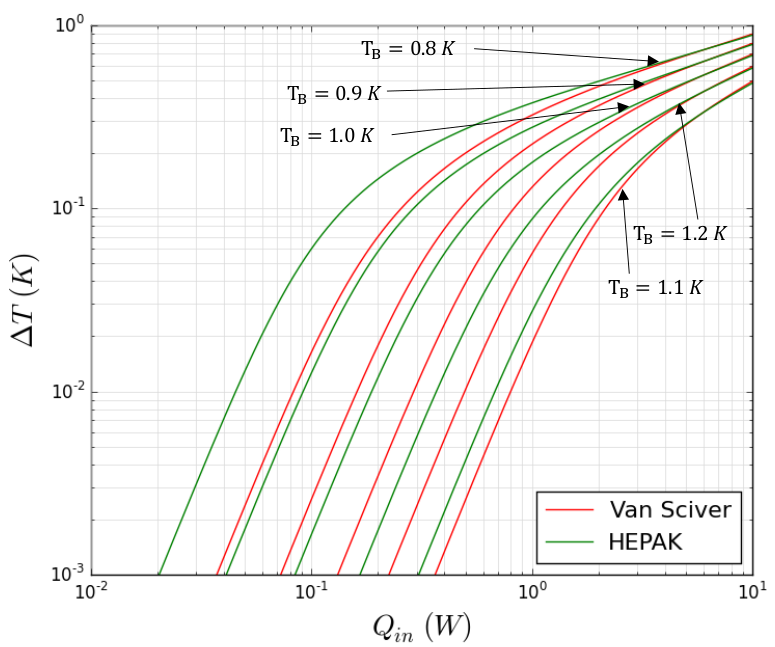
\includegraphics[width=0.8\textwidth]{VanSciver_vs_HEPAK.png}
  \caption{The heat conductivity function of the Van Sciver and HEPAK
    models. The vertical axis shows the temperature gradient along the
    channel and the horizonal axis shows the input heat
    flux~\cite{Florian_thesis}. The arrows on the graph indicate the
    temperature of the superfluid helium}
\label{fig:VanSciver_vs_HEPAK}
\end{figure}

The heat conductivity function for the Van Sciver and the HEPAK
theoretical models are shown in Fig.~\ref{fig:VanSciver_vs_HEPAK}. As
the graph shows, both models tend to agree at higher heat
inputs. However, at lower heat inputs, the heat conductivity function
values for the Van Sciver model lie below the values for the HEPAK
model. In addition, as the temperature of the superfluid helium
increases, the heat conductivity function tends to look more
linear. Since the Van Sciver model is more well known, it is used for
comparision with experimental data.

%%%%%%%%%%%%%%%%%%%%%%%%%%%%%%%%%%%%%%%%%%%%%%%%%%%%%%%%
\section{Measurement Result}
The data shown in Table.~\ref{tab:heattest} is a set of cleaned data
from all the heat tests in 2017. If the heat load on the cryostat is
higher than its cooling power, the temperature of the superfluid
helium would increase linearly without reaching an equilibrium. This
phenomena has been observed for higher heater powers e.g. 1~W. As a
result, that data is discarded.


Fig.~\ref{fig:April_Data} shows the result of the April heat test.
For a given heat input, the temperature difference between the base
and the saturation temperature for each temperature sensor is
calculated~(see table~\ref{tab:heattest}). The average of all of those
temperature differences give the overall $\Delta T$ across the
channel. Those are shown with black dots in Fig.~\ref{fig:April_Data}
as the raw data. However, the heat input for each data point should be
corrected since the total heat input is a combination of the added
heat from the heater tapes and the background heat load on the
cryostat which is not taken into account.


\begin{figure}[h!]
  \centering 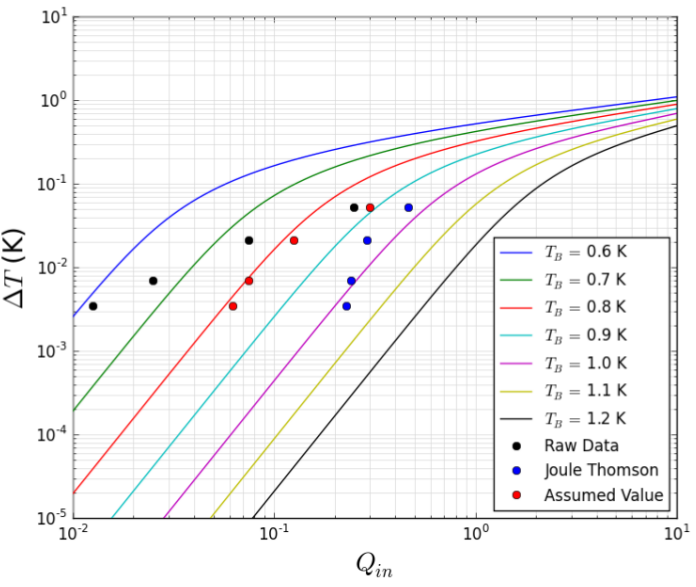
\includegraphics[width=0.8\textwidth]{April_Data.png}
  \caption{The comparison between the April heat test data and the Van
    Sciver model. The lines show the Van Sciver model's heat
    conductivity function at different superfluid helium bath
    temperatures. The black data points show the measured raw data of
    the heat tests. The blue points are the Joule Thomson values,
    which are the raw data plus the calculated background heat
    (included Joule-Thomson effect) and the red points show the raw
    data with the assumed 50 mW background heat input. }
\label{fig:April_Data}
\end{figure}


The two other sources of heat input to be considered are the
Joule-Thomson expansion and the the background heat load to the $^3$He
pot due to the thermal readiation and to the superfluid helium
bottle. The Joule-Thomson expansion happens when a gas or liquid
passes through a valve which has different temperature and pressures
on both sides while there is no heat exchange to the environment. Here
$^3$He flows into the heat exchanger and passes through a valve with
different pressures and temperatures on two sides. Because of the
Joule-Thomson expansion some liquid changes into vapor which is then
directly pumped out of the system and does not contribute to the
cooling process. For the backround heat load, based on estimations of
the sources of the background heat to the bottle alone, combined with
the measurements of the mass flow of $^4$He from the top of the bottle
when the $^3$He system is switched off, a heat of $\simeq$~50~mW is a
reasonable estimate of the true background heat to the bottle
alone. In Fig.~\ref{fig:April_Data}, the assumed values are the sum of
the 50~mW background heat and the heat input from the heaters and the
Joule-Thomson values are the sum of the heat input from the heaters
plus the calculated 232~mW calculated background
heat~\cite{Florian_thesis}.



Fig.~\ref{fig:November_Data} shows the data with the heaters in
November as well as the theoretical model of Van Sciver for the heat
conductivity. Each color represents a temperature range. The markers
are the actual data taken in November 2017.

At all the temperture ranges, the acquired data shows lower heat load
compared to the theoretical model. At the range of 1.2-1.3~K, the data
point with the smaller $\Delta$T is acquired at a higher He-II base
temperature, whereas the data point with higher $\Delta$T is acquired
at standard He-II base temperature. The data points which are closer
to the theoretical models are acquired at lower base temperature for
the superfluid helium. Since the measured data show bigger temperature
differences compared to the theoretical model of Van Sciver, it
suggests that the theory is assuming higher heat conductivity. Looking
back at Fig.~\ref{fig:VanSciver_vs_HEPAK}, it shows that using the
HEPAK model might solve this problem since the HEPAK model shows lower
heat conductivity.

One reason between the disagreement between the measurements and
theory could be the fact that these theoretical models are only
measured down to 1.4~K and they are extrapolated to lower
temperatures. Another reason could lie in the geometry difference. The
theoretical models are valid for a one-dimensional channel while there
is a 90$^\circ$ bend in the experimental setup~(see
Fig.~\ref{what???}) which can cause a higher temperature differnece
across the channel. One other reason might be the uncertainty in the
measured temperature due to the calibration of the temperature
sesnors. There might be other unknown sources of systematic error
affecting the measurements.


\begin{figure}[h!]
  \centering 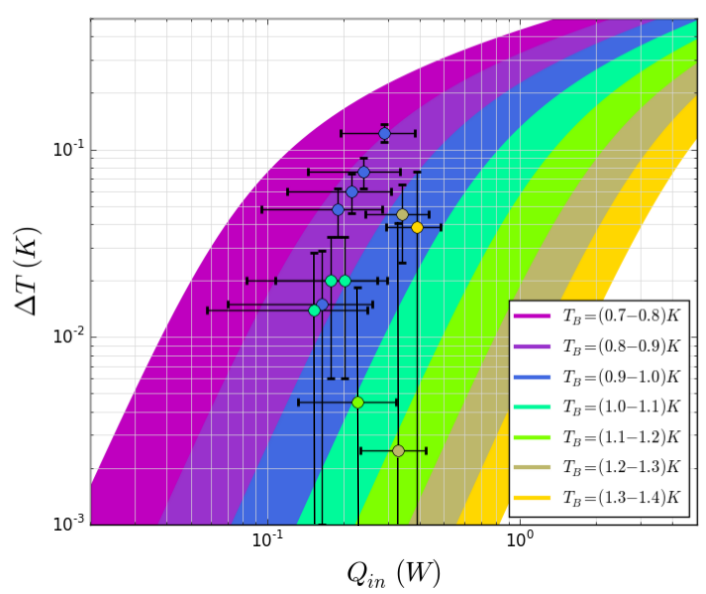
\includegraphics[width=0.8\textwidth]{November_Data.png}
  \caption{Theoretical model of Van Sciver for the heat conductivity
    at different temperature ranges and the November data. The
    vertical axis shows the temperature difference between the base
    and the saturation temperature for temperature sensors. The
    horizontal axis shows the heat input from the heaters plus the
    background heat.}
\label{fig:November_Data}
\end{figure}
